\documentclass{article}
\usepackage[utf8]{inputenc}
\usepackage[margin=3cm]{geometry}
\title{CSEN 901: Introduction to Artificial Intelligence \\Projct 1: Water Sort}
\author{Project Report \vspace{24pt} \\ Abdelrahman Aboelkehir, Hossain Ghoraba, \\ Mahmoud Aboelenein, Omar Hesham}
\date{18.10.2024}


\usepackage{natbib}
\usepackage{graphicx}
\usepackage{dirtree}
\usepackage{algorithm}
\usepackage{algpseudocode}

\begin{document}

\maketitle

\section{Introduction}
This project is the implementation of a search agent to solve the water sort puzzle. You can find a description of the water sort puzzle in the document titled \textbf{Project Description.pdf}. The agent is implemented in Java. The search the agent performs does not prune any branches early, nor does it perform any checks for whether the current node can or can not lead to a solution. A branch in the search is terminated only when there are no more possible nodes to expand from the leaf of that branch (in this probelm, this means there are no possible pour combinations to apply to the current state). The search terminates when either \textbf{a.} A node selected for expansion is identified as a goal state, or \textbf{b.} No more nodes on the search frontier can be expanded.

\newpage

\section{Project Hierarchy}

Here is a hierarchy of all the project files:

\dirtree{%
.1 src.
.2 main.
.3 java.
.4 code.
.4 generic.
.5 QueueingFunctions.
.6 QueueingFunction <<Interface>>.
.6 AStar1QueueingFunction.
.6 AStar2QueueingFunction.
.6 EnqueueAtEnd.
.6 EnqueueAtFront.
.6 EnqueueAtFrontWithDepthLimit.
.6 GREEDY1QueueingFunction.
.6 GREEDY2QueueingFunction.
.5 FixedSizeStack.
.5 Operator <<Interface>>.
.5 OperatorResult.
.5 Problem.
.5 SearchState.
.6 OrderedInsert.
.4 utils.
.5 ConditionalPrintStream.
.5 Methods.
.5 WaterSortUtils.
.4 watersort.
.5 Bottle.
.5 Color.
.5 LayerGroup.
.5 Pour.
.5 WaterSortProblem.
.5 WaterSortState.
.5 WaterSortUtils.
.4 GenericSearch.
.4 Node.
.4 WaterSortSearch.
}

\newpage

\begin{figure}[t]
\section{Class Diagram}
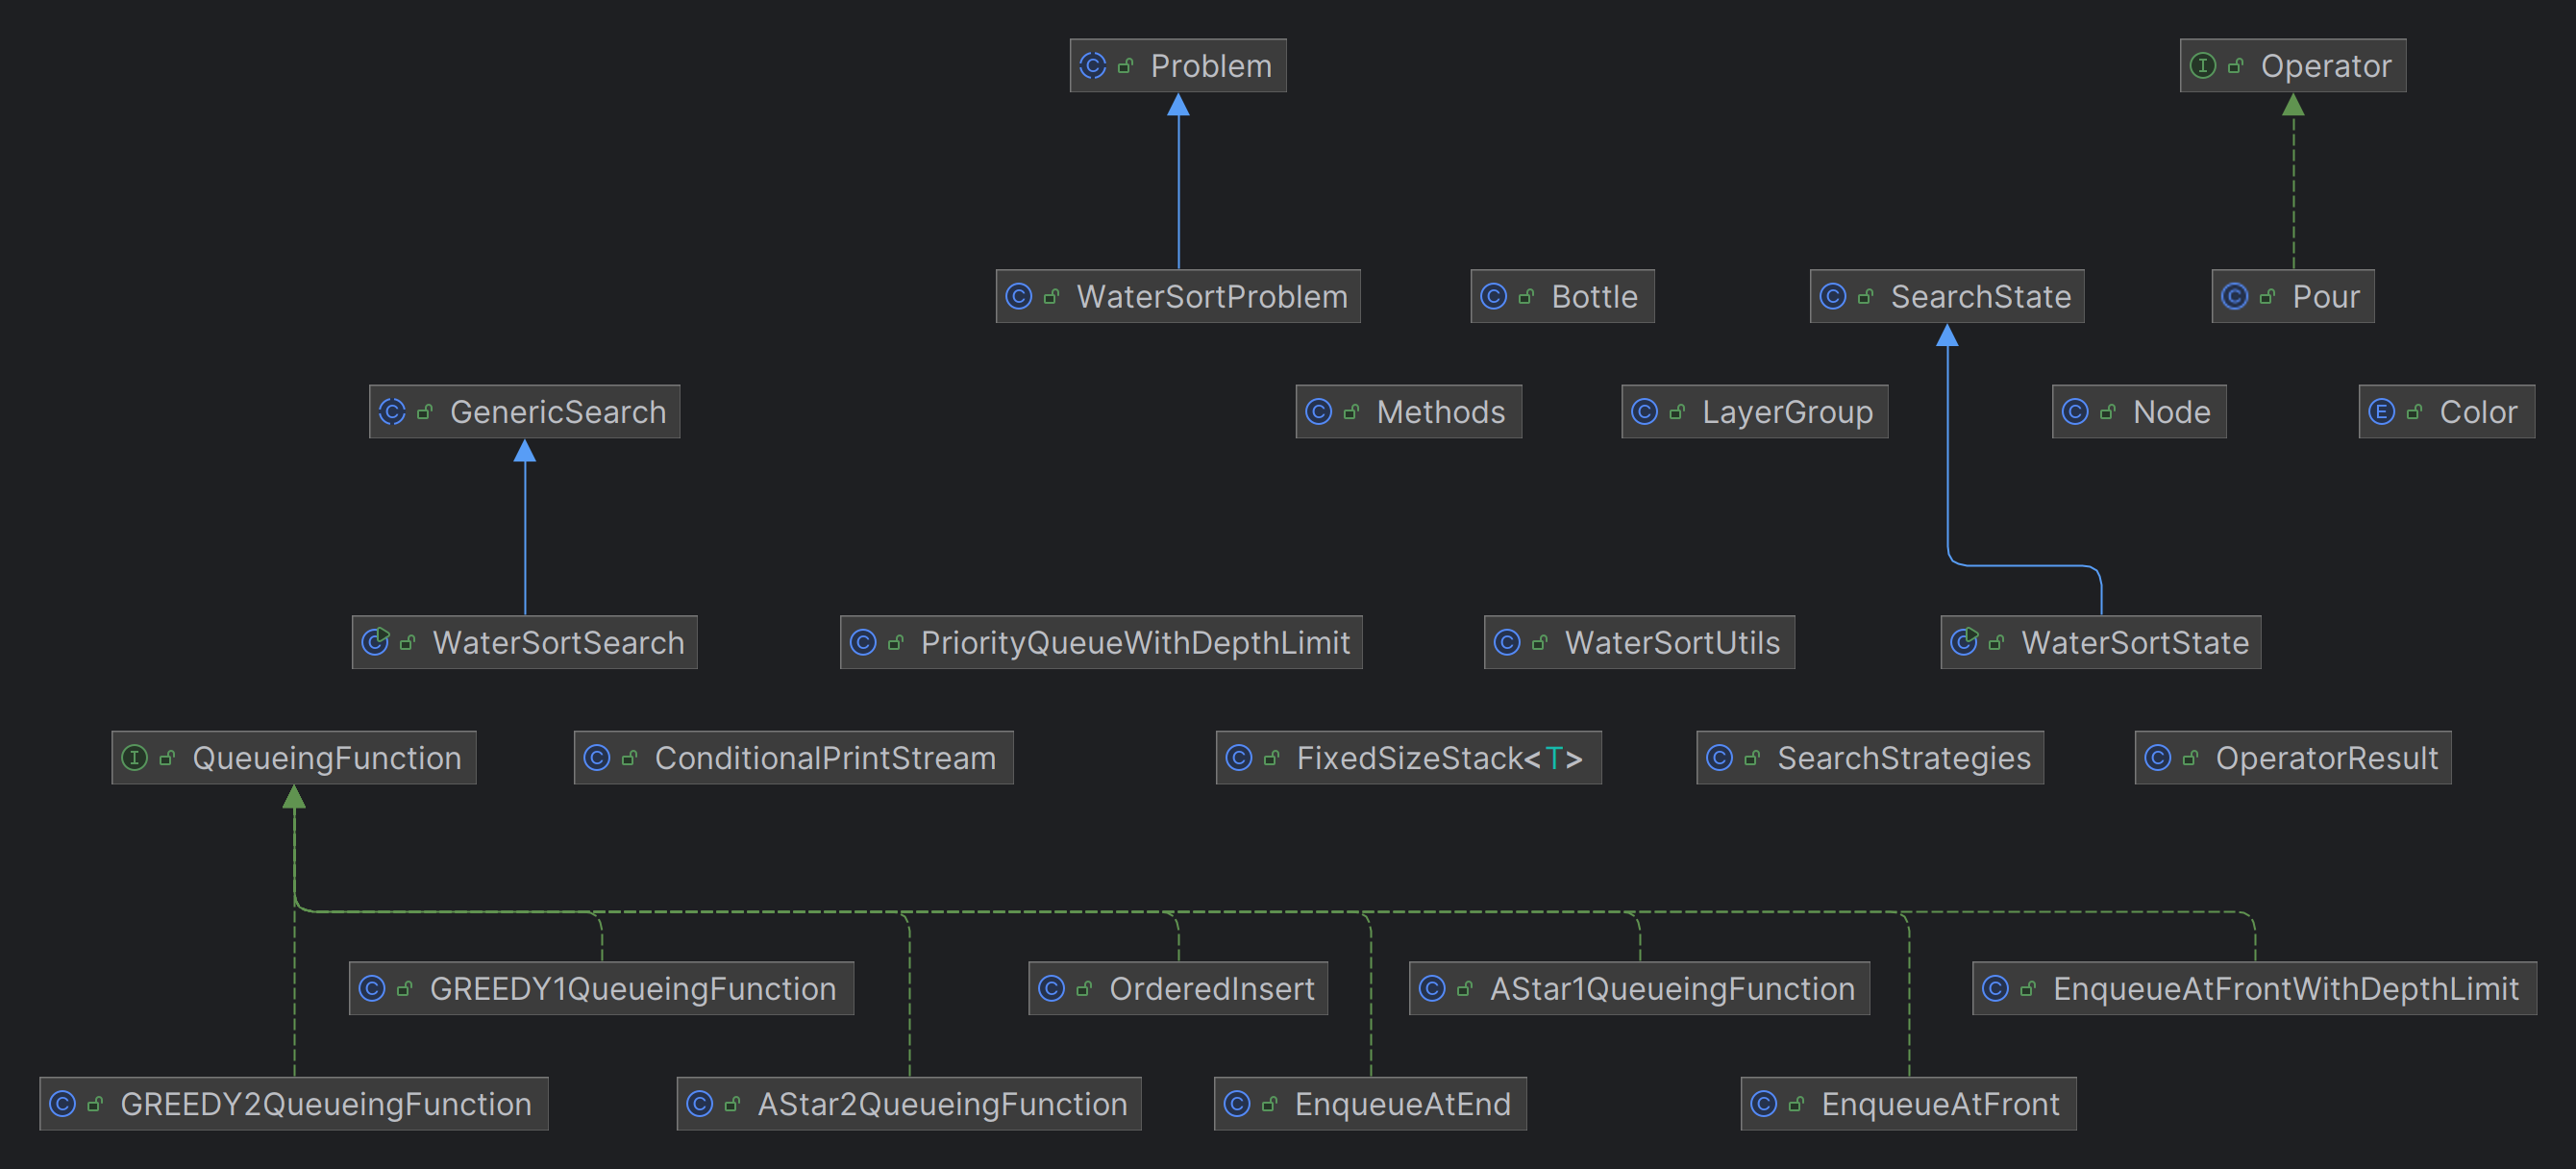
\includegraphics[scale=0.18]{Class Diagram.png}
\caption{Class Diagram}
\end{figure}

\section{Implementation of the Search Algorithms}

Our implementation for all search algorithms closely follows the description of the \textsl{GeneralSearch} algorithm outlined in lecture 2 of the course: 


\begin{algorithm}
\caption{GENERAL-SEARCH(problem, QING-FUN)}
\begin{algorithmic}[1]
    \State \textbf{return} a solution, or failure
    \State $nodes \gets \texttt{MAKE\_Q}(\texttt{MAKE\_NODE}(\texttt{INIT\_STATE}(problem)))$
    \While{true}
        \If{$nodes is empty$}
            \State \textbf{return} failure
        \EndIf
        \State $node \gets \texttt{REMOVE\_FRONT}(nodes)$
        \If{$\texttt{GOAL\_TEST}(problem)(\texttt{STATE}(node))$}
            \State \textbf{return} node
        \EndIf
        \State $nodes \gets \texttt{QING\_FUN}(nodes, \texttt{EXPAND}(node, \texttt{OPER}(problem)))$
    \EndWhile
\end{algorithmic}
\end{algorithm}

All the algorithms use a Java \texttt{PriorityQueue} as their queue. The \texttt{PriorityQueue} in Java orders objects based on a given \texttt{Comparator}. The classes in the \texttt{QueueingFunctions} package return a \texttt{Comparator}, which, according to the search strategy being used, orders the elements in the queue in a certain manner. This  \texttt{Comparator} is then used to initialize a queue. \\

\newpage

For example, here is the queuing function for Breadth-First Search: 

\begin{verbatim}
public class BFSQueuingFunction implements QueuingFunction {
  @Override
  public Comparator apply() {
    return new Comparator.comparingInt(Node::getDepth);
  }
}
\end{verbatim}

In this case, when a \texttt{PriorityQueue} is created using the returned \texttt{Comparator}, all the nodes in the queue will be ordered in ascending order of depth.
\end{document}